\subsection{Modelli ad Agente}
% scrivere sezione simile ad articolo (download)
Un modello ad agente e' un modello computazionale per la simulazione delle 
azioni e interazioni di un insieme di agenti autonomi, siano essi individui
o gruppi di individui, con l'obiettivo di comprendere il comportamento 
del sistema e la relazione che vige con i suoi risultati \cite{wiki:Agent-based_model}
\cite{7822080}.

\begin{minipage}{\linewidth}
    \centering
    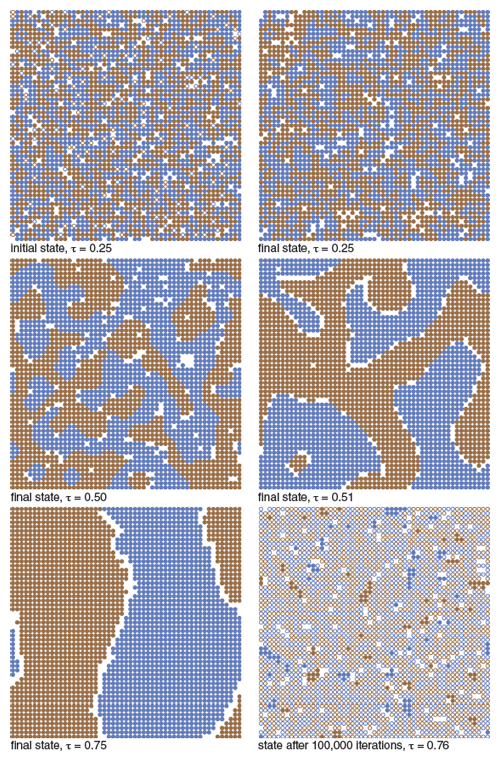
\includegraphics[scale=0.5]{img/201381146479794-2013-09HayesF1png.png}
    \captionof{figure}{Schelling's model of segregation simulato tramite ABM}
    \label{fig:schelling_segregation_abm}
\end{minipage}

L'utilizzo di modelli ad agente in epidemiologi e' una tecnica nota che 
da piu' di un decennio viene impiegata per simulare e comprendere le 
situazioni e i problemi piu' disparati, tutti pero' generalmente accomunati
dal fatto che come parametro portante vi sia il comportamento umano \cite{Groff2019}
\cite{El-Sayed2012-ac} \cite{Tracy2018-lc} \cite{Bissett2021}. 
Uno dei parametri piu' caratterizzanti che da sempre sono stati tenuti 
in considerazione e assunti come ristretti ad una piccola cerchia, sono 
le interazioni sociali tra individui. Questo sovrainsieme di parametri 
racchiude molteplici sottoinsiemi di parametri che descrivono delle 
interazioni piu' specifiche ma che possono essere raggruppate come macro 
categoria se si scende a compromessi. 

Questa specifica e' importante in quanto uno delle sfide piu' grandi che 
il mondo della simulazione, e quindi quello epidemiologico devono affrontare
e' proprio quello di trovare un modo efficiente e soprattutto realistico 
di simulare le interazioni sociali tra individui, in quanto queste possono
influenzare notevolmente i risultati di una simulazione definendola utile
oppure inutile \cite{Silverman2021}. Non soltanto, un'altra sfida e' il modo 
con cui si decide di rappresentare lo spazio (e il tempo) all'interno della
simulazione. In base al tipo di discretizzazione effettuata una simulazione
potrebbe essere utile in un campo ma totalmente inutile in un altro 
\cite{KONSTANTINOUDIS2020100319}.

\begin{minipage}{\linewidth}
    \centering
    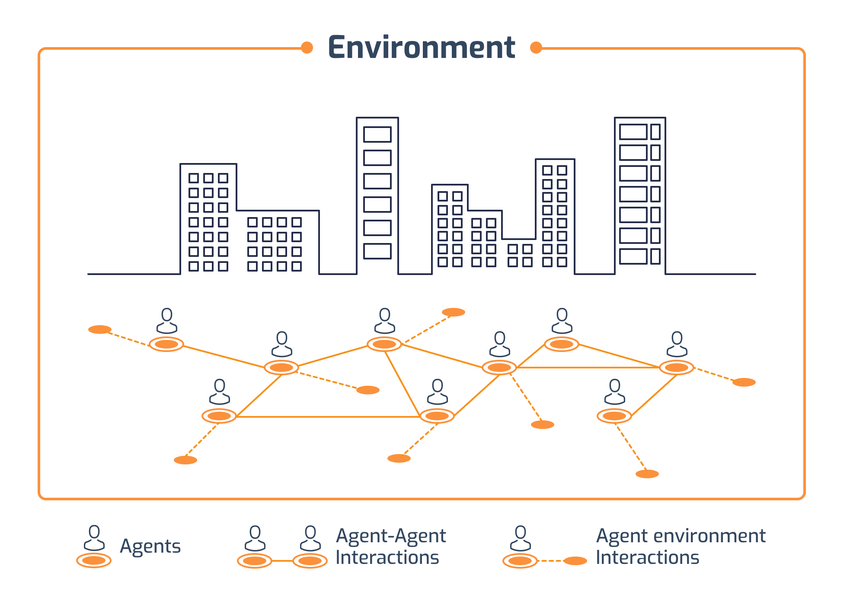
\includegraphics[scale=0.5]{img/Schematic-representation-of-an-agent-based-model-ABM.png}
    \captionof{figure}{Rappresentazione schematica di un modello ad agente}
    \label{fig:schematic_representation_abm}
\end{minipage}

Con l'arrivo della pandemia da COVID-19 molti ricercatori hanno 
focalizzato la propria attenzione sull'idea di sviluppare un modello 
ad agente puro oppure ibrido \cite{Marzban2021-pd}
(ibridato con delle ODE oppure delle Partial DE), con l'obiettivo di 
trovare un modello di simulazione in grado di simulare in maniera 
affidabile il decorso di una pandemia tenendo in considerazione le 
variabili piu' stocastiche e imprevedibili come il comportamento umano.
L'ambiente di lavoro simulato era generalmente un ambiente controllato
che poteva essere una citta' come in \cite{PRAJAPATI20232299}, 

Un'altro obiettivo e' quello di osservare l'impatto degli interventi non 
farmaceutici sulla popolazione come riporta \cite{NOVAKOVIC2022108790}
\cite{10.1371/journal.pcbi.1009149}.
Altri ancora invece utilizzano l'approccio simulativo tramite modelli ad 
agente per estrapolare delle ODE tramite l'analisi del modello, come
riportato da \cite{Nardini2021-pu}. 

\subsubsection{Discretizzazione}
La tematica della discretizzazione e' una delle proprieta' fondamentali
e al contempo uno dei problemi atavici della simulazione.
Il mondo in cui viviamo e' un mondo continuo, ma gli strumenti
che attualmente abbiamo per simularlo sono discreti, per cui 
ogni qualvolta che vogliamo simulare un evento dobbiamo decidere 
in che modo adattare la realta' alla simulazione, andando 
inequivocabilmente a perdere informazioni nel processo 
\cite{KONSTANTINOUDIS2020100319}. 

\begin{minipage}{\linewidth}
    \centering
    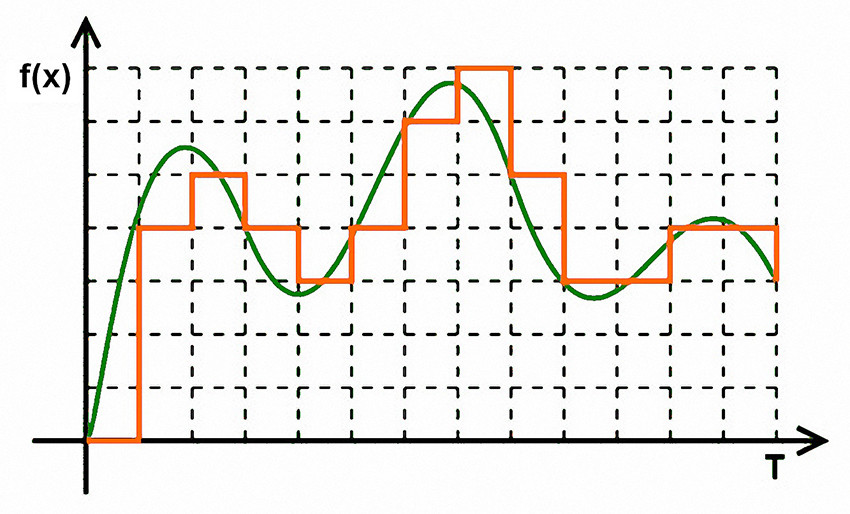
\includegraphics[scale=0.5]{img/figura-1-analogico-e-digitale-7ae2c4b25c8751e9a3771f91f1e65bb1f.jpg}
    \captionof{figure}{Esempio di discretizzazione dei dati}
    \label{fig:discretization}
\end{minipage}

Il processo di discretizzazione in una simulazione puo' prendere 
principalmente due macro aree che sono: lo spazio e il tempo. 
Molti framework di simulazione implementano al loro interno 
diversi trucchetti per simulare in maniera quanto piu' accurata
un insieme di dati continuo, permettendo all'utente di utilizzare
parole chiave come ad esempio ContinuousSpace. Quello che praticamente
viene fatto e' creare un ambiente per il modello che e' il piu'
preciso e granulare possibile, per cui servono allo scopo fintanto
che quest'ultimo non richiede una maggiore precisione. 

Il processo di discretizzazione comunque non e' sempre negativo, 
in quanto alcuni problemi possono essere simulati in maniera 
estremamente fedele anche effettuando questi accorgimenti, e anzi
alle volte non e' perfino necessario avere una precisione troppo 
alta per la simulazione di determinati eventi.

Se ad esempio si volesse simulare tramite un agente una partita 
a Risiko, non e' necessario richiedere uno spazio e un tempo continuo
della simulazione, in quanto questi possono essere rimpiazzati 
dalla loro controparte discreta che sono caselle e turni. 

\begin{minipage}{\linewidth}
    \centering
    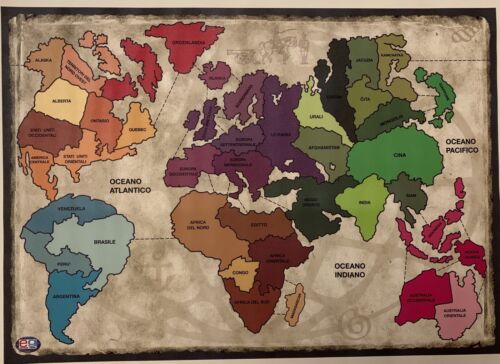
\includegraphics[scale=0.5]{img/s-l500.jpg}
    \captionof{figure}{Plancia di gioco di Risiko}
    \label{fig:risiko}
\end{minipage}

Se si volesse simulare il traffico aereo si potrebbe utilizzare
uno spazio a grafo dove ogni nodo rappresenta un aeroporto e 
gli archi rappresentano la tratta in partenza o in arrivo. Anche in 
questo caso l'applicazione della discretizzazione non sarebbe 
qualcosa di problematico.